%!TEX root = ../Thesis.tex

\chapter{Metodología}\label{ch:chap5}

\epigraphhead[70]{
\epigraph{There was nowhere to go but everywhere, so just keep on rolling under the stars.}
{Jack Kerouac}}

A continuación se describe la metodología usada para 

\section{Esquema general} 

Agregar esquema de la metodología que se siguió.

\begin{figure}[bth]
  \centerline
  {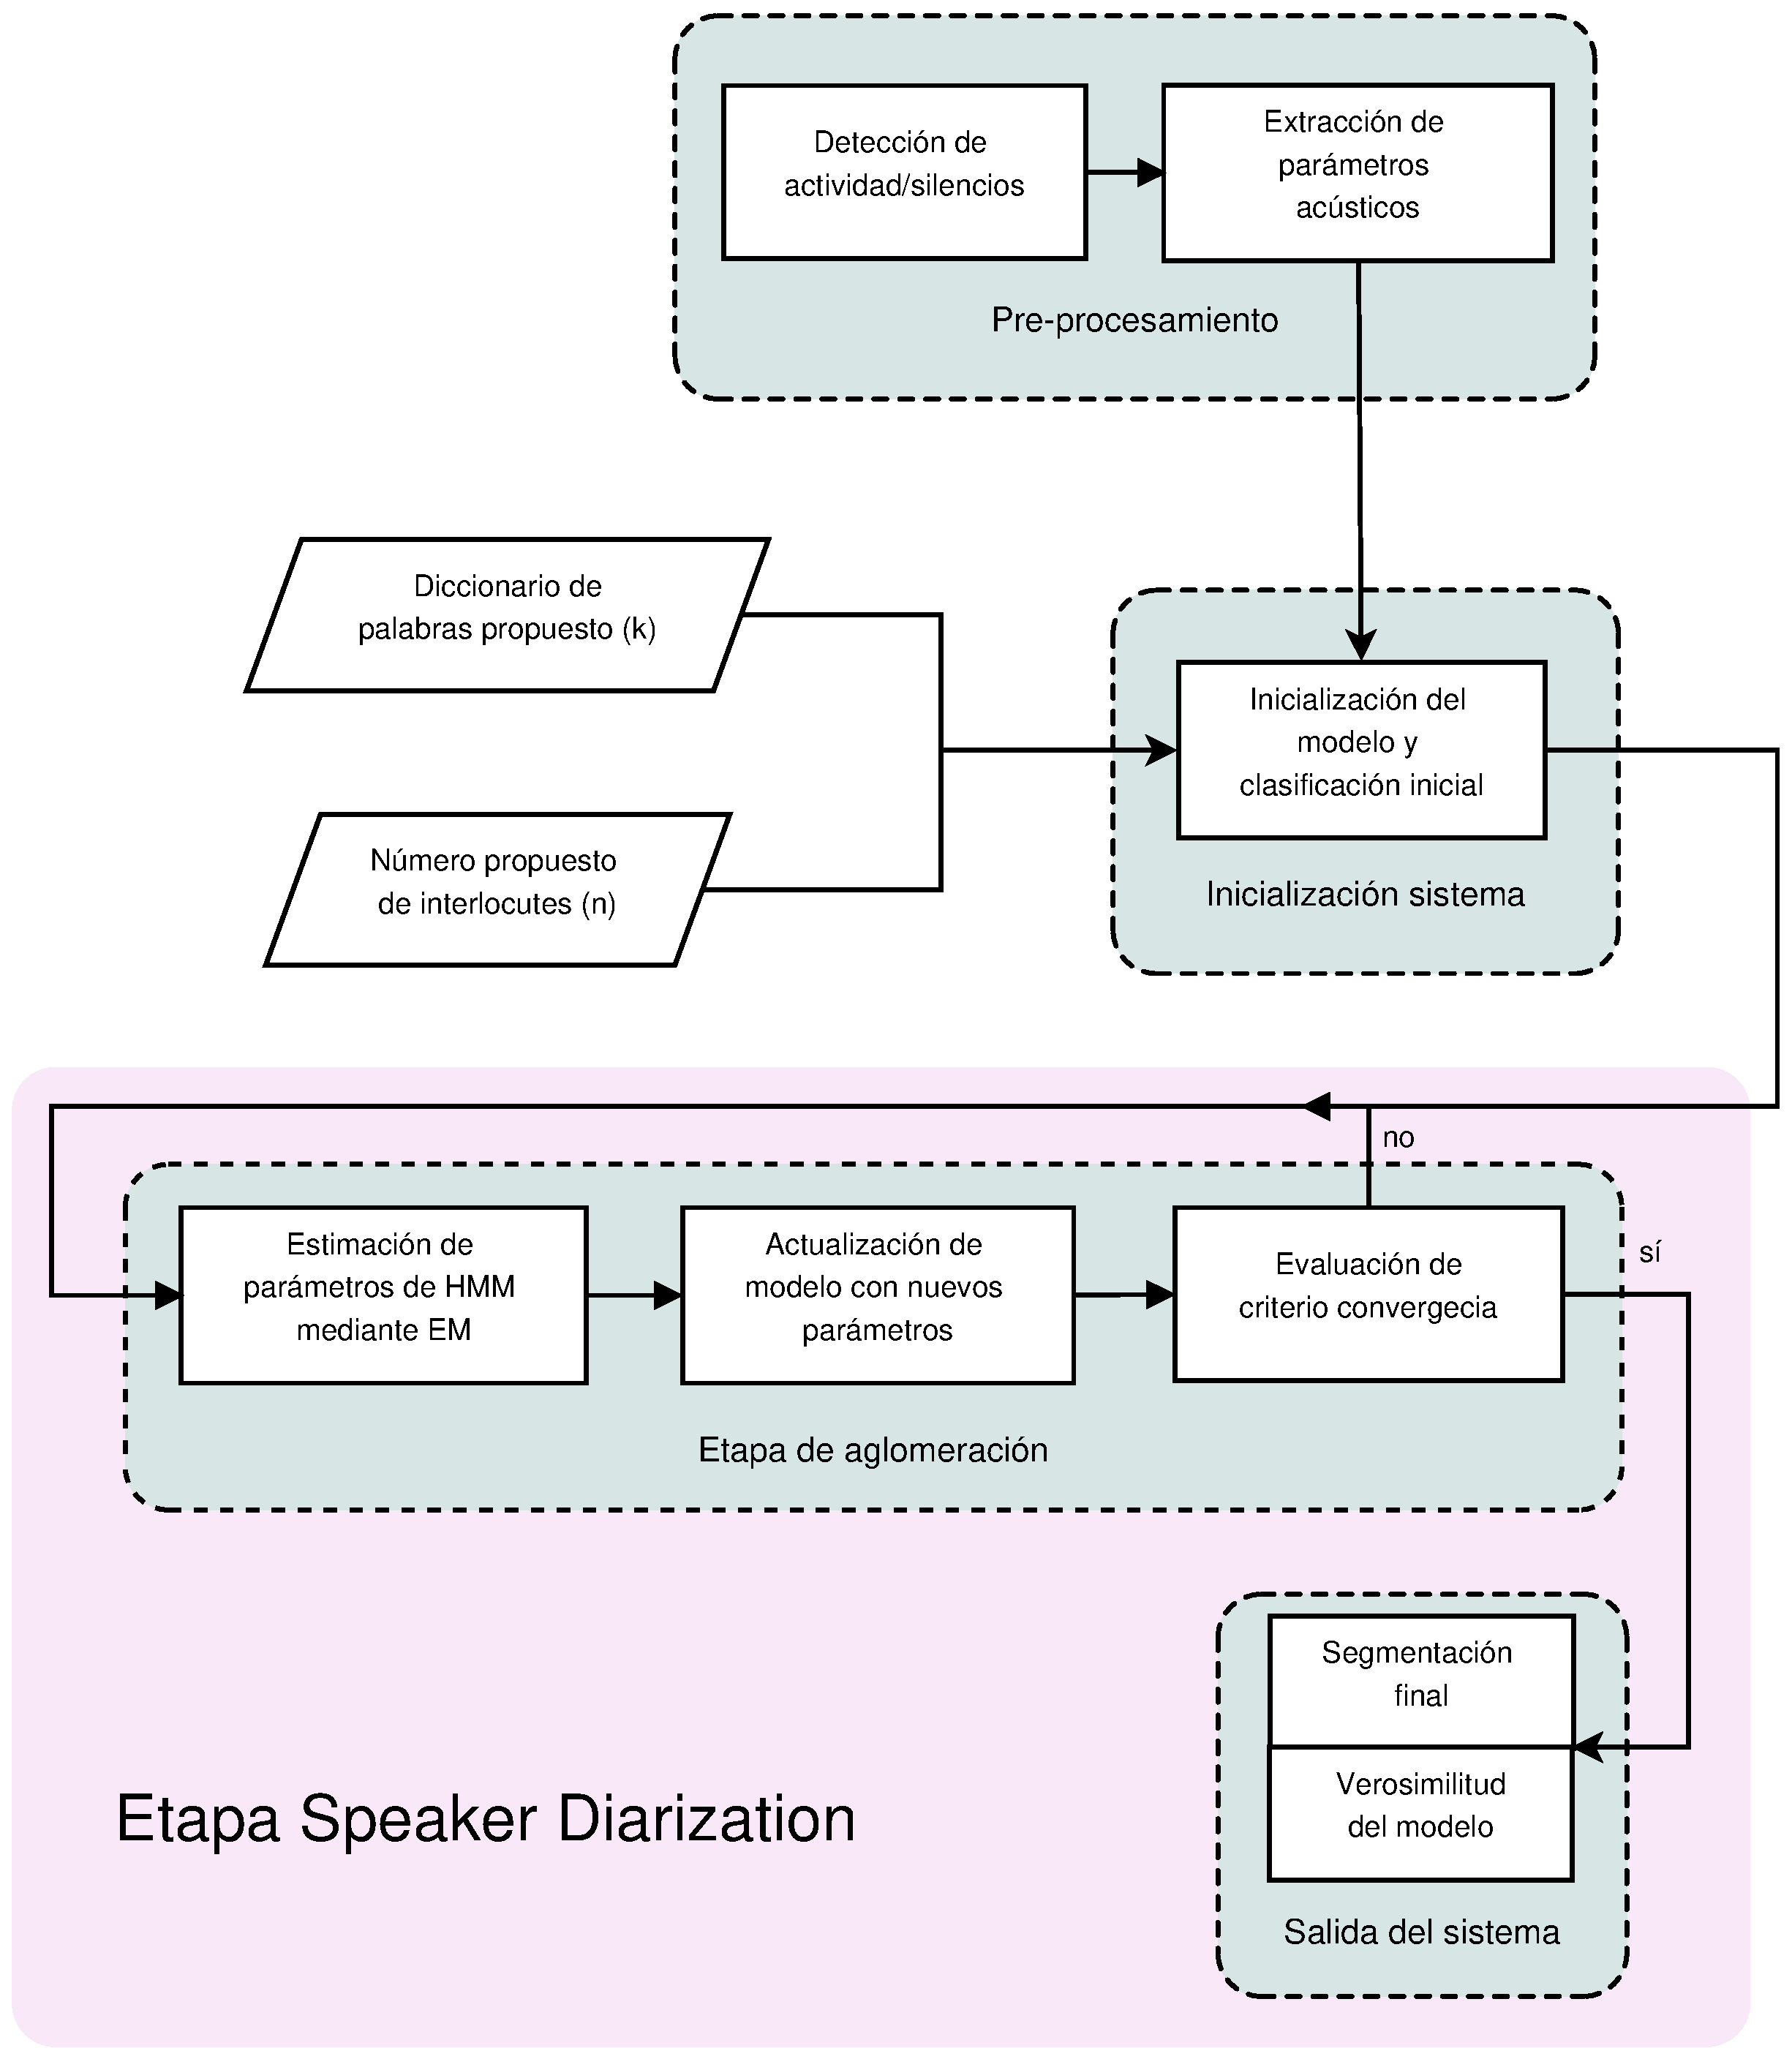
\includegraphics[width=1.5\linewidth]{gfx/chap5/general_flow}} \quad
  \caption{Esquema general.}
  \label{fig:esquema}
\end{figure}

\section{Resolver modelo HMM usando EM} 
\label{sec:sd-hmm-em}

La metodología propuesta se puede observar 

Para las pruebas que se han realizado hasta ahora, se han usado grabaciones creadas sintéticamente; esto es, usando un sintetizador de voz. El hacer las grabaciones con voces sintéticas nos permite tener un mayor control sobre la calidad de la grabación (no hay ruidos aditivos o interferencias), además de poder generar muchos más casos de prueba sin tantas complicaciones.
